\section{Gradient Descent} \label{sec:prob1}
In this section, we implemented Gradient Descent in Python to find the minimum of a function.

\subsection{Part 1}
Our Gradient Descent (GD) implementation begins with an initial guess, $x_0$, of the argument $x_{min}$ that minimizes the function, $f(x)$.
The implementation is applied to two functions, a negative Gaussian and a quadratic bowl.
The gradient, dfdx, can be calculated in closed form (for simple functions), and the next estimate of $x_{min}$ is updated according to the rule $x_{i+1} = x_i - \alpha \cdot \frac{\partial f(x_i)}{\partial x}$.
Here, $\alpha$ is the step size, or learning rate, which controls how much the gradient affects the next estimate.
The rule is applied until either a pre-determined maximum number of iterations, $n_{iters}$, occurs, or the function's value at the current iteration differs from the previous iteration's estimate by less than $\epsilon$.
Each of these paramters, ($\alpha$, $n_{iters}$, and $\epsilon$) impact the GD solution in different ways.

In~\cref{fig:initial_guess}, the intial guess, $x_0$, is varied to show that a close intial guess leads to convergence in only a few steps.
As the norm of difference between initial and final estimates grows, the number of iterations increases.
For certain initial guesses, we observed that the algorithm did not converge in some maximum number of iterations.
For the negative Gaussian, this is because the gradient is very small far from the mean.

The convergence limit determines when the GD algorithm stops, seen in ~\cref{fig:convergence}.
The error increases if $\epsilon$ is too large, as on the right of~\cref{fig:convergence1}.

In GD, the norm of the gradient decreases as the solution converges, which is shown for the quadratic bowl function in~\cref{fig:gradient}.


\begin{figure}
	\centering
	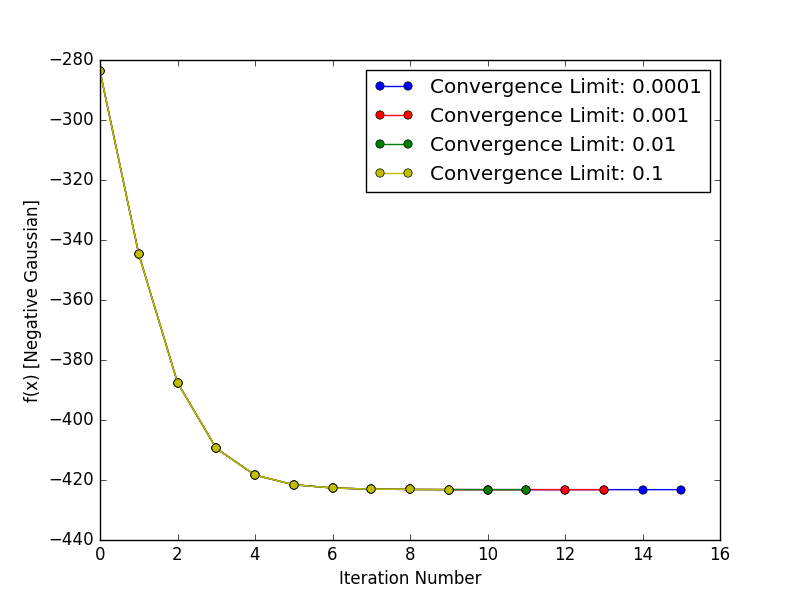
\includegraphics [trim=0 0 0 0, clip, angle=0, width=0.8\columnwidth,
	keepaspectratio]{figures/1_1_convergence1}
	\caption{As convergence limit, $\epsilon$, increases, the iteration stops earlier. From this view, the four solutions differ very little.} 
	\label{fig:convergence1} 
	%\vskip -0.1in
\end{figure}

\begin{figure}
	\centering
	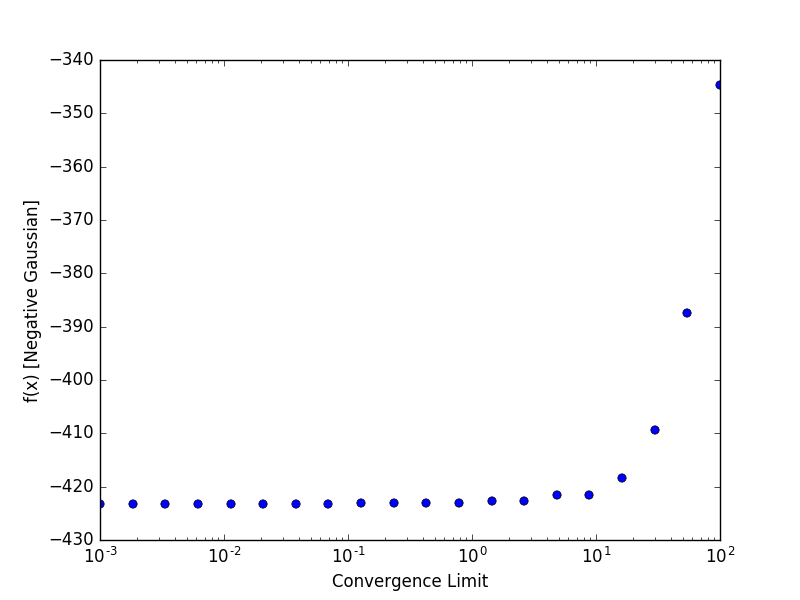
\includegraphics [trim=0 0 0 0, clip, angle=0, width=0.8\columnwidth,
	keepaspectratio]{figures/1_1_convergence}
	\caption{The final value returned by GD can differ substantially if convergence limit is set too loosely.} 
	\label{fig:convergence} 
	%\vskip -0.1in
\end{figure}

\begin{figure}
	\centering
	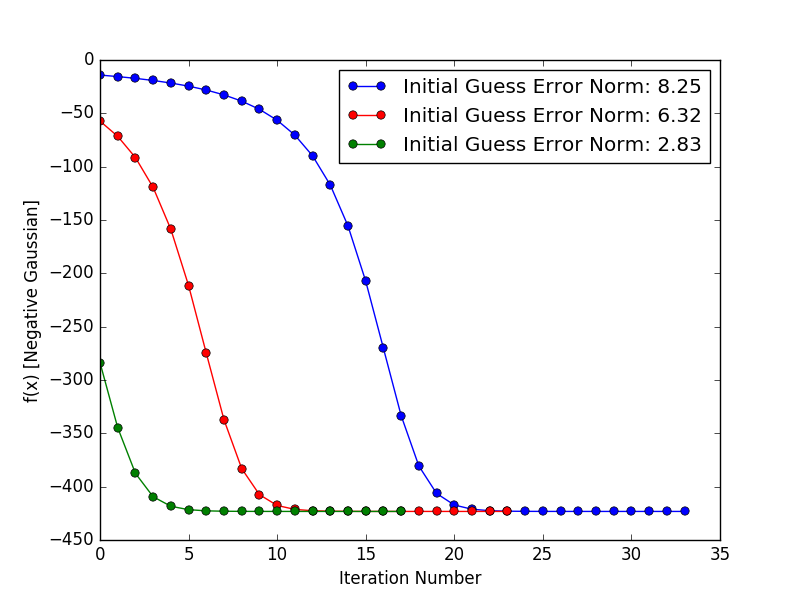
\includegraphics [trim=0 0 0 0, clip, angle=0, width=0.8\columnwidth,
	keepaspectratio]{figures/1_1_initial_guess}
	\caption{When initial guess is far from true minimum, it takes many iterations (blue) to converge. As initial guess approaches final solution, number of iterations decreases.} 
	\label{fig:initial_guess} 
	%\vskip -0.1in
\end{figure}

\begin{figure}
	\centering
	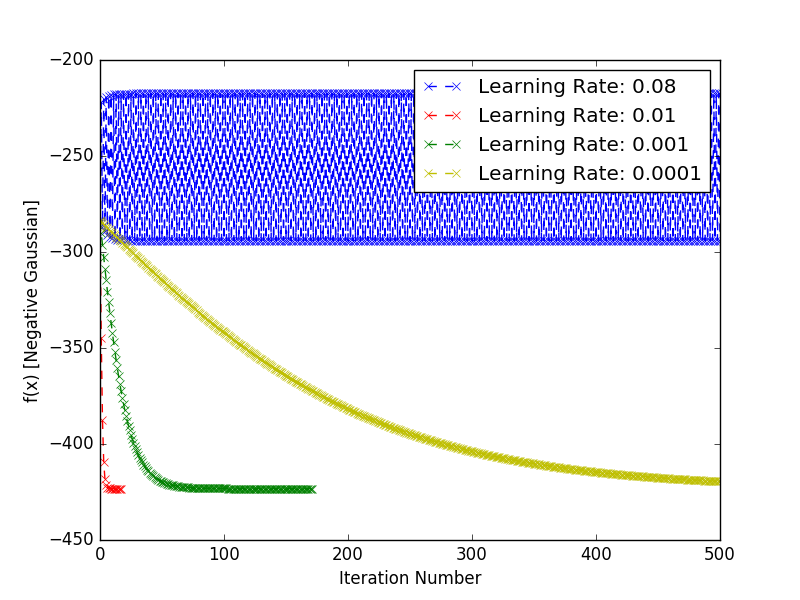
\includegraphics [trim=0 0 0 0, clip, angle=0, width=0.8\columnwidth,
	keepaspectratio]{figures/1_1_step_size}
	\caption{If learning rate, $\alpha$, is too large (blue), the solution will oscillate or diverge each iteration. If $\alpha$ is too small, it will take many iterations to converge (yellow). Convergence takes only a few iterations for proper $\alpha$ (red).} 
	\label{fig:learning_rate} 
	%\vskip -0.1in
\end{figure}

\begin{figure}
	\centering
	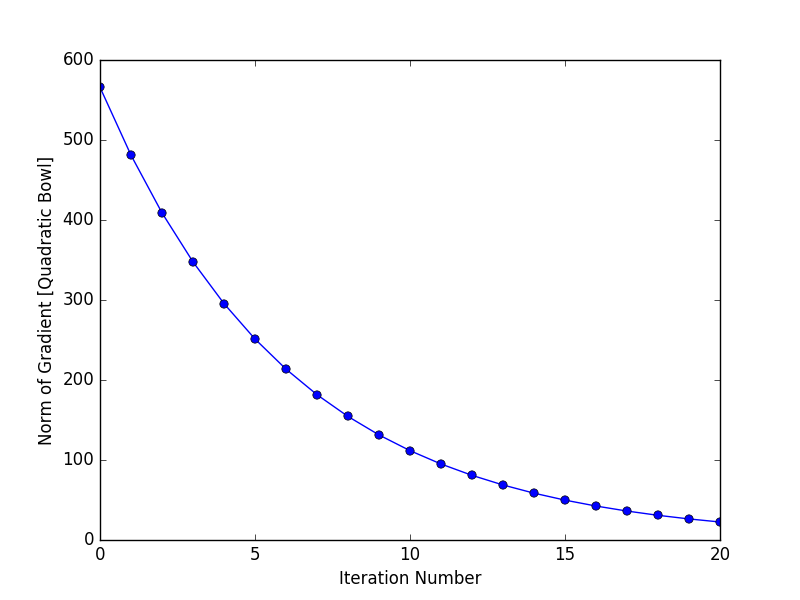
\includegraphics [trim=0 0 0 0, clip, angle=0, width=0.8\columnwidth,
	keepaspectratio]{figures/1_1_gradient}
	\caption{Norm of gradient decreases with each iteration in GD. This example minimizes the Quadratic Bowl function.} 
	\label{fig:gradient} 
	%\vskip -0.1in
\end{figure}











